\documentclass[12 pt]{article}
\usepackage{amsmath}
\usepackage{url}
\usepackage{graphicx}
\usepackage{setspace}
\usepackage{pgf}
\usepackage{tikz}
\usetikzlibrary{arrows,automata}
\usepackage[latin1]{inputenc}
\usepackage{verbatim}
\usepackage[margin=1.2in]{geometry}

%	\addtolength{\oddsidemargin}{-.5in}
%	\addtolength{\evensidemargin}{-.5in}
%	\addtolength{\textwidth}{0.75in}
%	\addtolength{\topmargin}{-1in}
%	\addtolength{\textheight}{1.75in}
\title{Final Year Project Interim Report\\ Predicting Web 2.0 Thread Updates}
\author{U096883L Shawn Tan}
\date{}
\begin{document}
\doublespacing
\maketitle
\section{Introduction}
With the advent of Web 2.0, sites with forums, or similar thread-based discussion features are increasingly common.
In this project,our goal is to predict updates in such threads.
%Just recently, Google+ has just



\begin{table}\label{table:web20}
	\makebox[\textwidth][c]{
	{\footnotesize
	\begin{tabular}{|l|c|c|c|c|c|c|c|c|c|c|}
		\hline
			\input{web20}
		\hline
	\end{tabular}
	~\\
	}
	}
	{\footnotesize
\caption{Features of popular Web 2.0 sites}
	\begin{tabular}{l l}
		T &= Twitter mentions\\
	 FB L &= Facebook Likes \\
		FB S &= Facebook Shares\\
	G +1 &= Google +1\\
		   L&= Likes (Local) \\
   		DL &= Dislikes (Local) \\
			C &= Comments \\
		PV &= Page Views \\
   Follows &= Site-local feature for keeping track of user's activities
	\end{tabular}
}
\end{table}

Table \ref{table:web20} shows us that many of the popular Web 2.0 sites have comment features. This suggests that content on the web is increasingly being created by users alongside content providers. While mining structured, curated content from sites like Amazon, for data like prices is easy and effective, data that can be obtained from user-generated content are of a different nature. One may be able to infer public sentiment about a given product that would not be readily available from an e-commerce site.
%we are predicting web 2.0 updates
In some cases, news may travel more quickly through such online community discussion than through traditional media. Users also typicaly discuss purchased products bought online via these forums, and companies that want to get timely feedback about their product should turn to data mined from such sites.

A naive way of getting timely updates is to aggressively hit the pages repeatedly downloading the pages at a very frequent rate. However, the number of pages in a forum site are far too large to perform this efficiently on every forum. One way to minimise this cost would be to look at the time differences between previous posts to estimate the arrival of the next one. We believe that the content of the thread has information that can give a better estimate of the time interval between the last post and a new one.


For example, a thread in a technical forum about a Linux distribution may start out as a question. Subsequent questions that attempt to either clarify or expand on the original question may then be posted, resulting in a quick flurry of messages. Eventually, a more technically savvy user of the forum may come up with a solution, and the thread may eventually slow down after a series of messages thanking the problem solver. Suppose 10 days later, someone with a slight variation of the same problem posts on the thread again. A crawler solely on the age of the thread to determine its download rate of the thread may not update itself with the thread.
%TODO:Bring to beginning and shorten to 1 or 2 sentences after the problem statement.
%as rate increase, timeliness become more important
% talk about consequences of naive method

Let us define all such thread-based discussion styled sites as forums. Ideally, an incremental crawler of such user-generated content should be able to maintain a fresh and complete database of content of the forum that it is monitoring. However, doing so with the previously mentioned naive method would (1) incur excessive costs when downloading un-updated pages, and (2) raise the possibility of the web master blocking the requester's IP address.

%Thus, we need a strategy of revisiting pages that will reduce the cost of downloading unchanged pages, while at the same time downloading them as soon as possible after it's update. 
This year-long project proposes to use content-based features of a given thread to predict its next update time. We argue, that the content within the posts of the thread should be important in predicting the thread updates, and propose our approach to solving the problem.

\section{Related work}

\subsection{Refresh policies for incremental crawlers}
In order to devise such a strategy, we need to predict how often any user may update a page. Some work has been done to try to predict how often page content is updated, with the aim of scheduling download times in order to keep a local database fresh.


We will discuss the \emph{timeliness} of our crawler to maintain the freshness of the local database, which refers to how new the extracted information is. Web crawlers can be used to crawl sites for user comments and threads for postprocessing later. Web crawlers which maintain the freshness of a database of crawled content are known as incremental crawlers. Two tradeoffs these crawlers face cited by Yang et. al. 2009 \cite{Yang2009} are \emph{completeness} and \emph{timeliness}. \emph{Completeness} refers to the extent which the crawler fetches all the pages, without missing any pages. \emph{Timeliness} refers to the efficiency with which the crawler discovers and downloads newly created content. We focus mainly on timeliness in this project, as we believe that timely updates of active threads are more important than complete archival of all threads in the forum site.

Many such works have used the Poisson distribution to model page updates. Coffman et. al. \cite{Coffman1997} analysed the theoretical aspects of doing this, showing that if the page change process is governed by a Poisson process $\lambda e^{-\lambda \mu}$, then accessing the page at intervals proportional to $\mu$ is optimal.

Cho and Garcia-Molina trace the change history of 720,000 web pages collected over 4 months, and showed empirically that the Poisson process model closely matches the update processes found in web pages\cite{Cho1999}. They then proposed different revisiting or refresh policies \cite{Cho2003,Garcia-molina2003} that attempt to maintain the freshness of the database.

The Poisson distribution were also used in Tan et. al. \cite{Tan2007} and Wolf et. al. \cite{Wolf2002}. %elaborate!!!!
However, the Poisson distribution is memoryless, and in experimental results due to Brewington and Cybenko \cite{Brian2000}, the behaviour of site updates are not. Moreover, these studies were not performed specifically on online threads, where the behaviour of page updates may be very different from that of static pages.

Yang et. al. \cite{Yang2009}, attempted to resolve this by using the list structure of forum sites to infer a sitemap. With this, they reconstruct the full thread, and then use a linear-regression model to predict when the next update to the thread will arrive. %elaborate!!!

Online forums and bulletins have a logical, hierarchical structure in their layout, which typically alerts the user to thread updates by putting threads with new replies at the very top of the thread index. Yang's work exploits this as well as their linear model to achieve a predicton of when to retrieve the pages.
However, this is not so for comments found on blog sites or discussion threads in an e-commerce site about a certain product and the lack of these pieces of information may result in a poorer estimate, or no estimate at all.


Our perspective is that the available content on the thread at the time of the retrieval should also be factored into the model used to predict the page updates. Next, we look at some of the related work pertaining to thread content.

\subsection{Thread content analysis}
While there is little existing work using content to predict page updates, we will review some existing work related to analysing thread-based pages which we think will aid us in our efforts to do content-based prediction.

Wang et. al \cite{Wang2011} did work in finding out linkages between forum posts using lexical chaining. They proposed a method to link posts using the tokens in the posts called $Chainer_{SV}$. While they do analyse the content of the individual posts, the paper does not make any prediction with regards to newer posts. The methods used to produce a numeric similarities between posts may be used as a feature to describe a thread in its current state, but incorporating this into our model is non-trivial.

%Kleinberg used Hidden Markov Models to predict ``bursts" in message arrival times \cite{Kleinberg2003}. In his running example, he used email messages, and used time between messages to estimate the states that produced the sequence. While the model may be able to predict what the state is for the next time interval, it does so using the history of message arrival times, and does not take into account the content within the messages themselves.


%One also cannot ignore the fact that social factors play a role when users interact in an online discussion. Granovetter's threshold model for social behaviour may also be useful in describing how the users behave as a whole.

With these related work in mind, we next propose our modelling of a thread as a Markov chain, and our approach to solving the problem.

\section{Approach}
Our objective is to minimise the cost of fetching pages, while still being able to keep our local database of pages updated. To this end, we model a thread as being governed by a Markov chain. In each state, a certain set of words and their frequencies will be emitted with certain probability. Each state has a certain probability of transitioning back to itself or to the other states after the next observation or refreshing of the thread.

We could modify Kleinberg's use of HMMs to detect bursts in his email stream \cite{Kleinberg2003}. Instead of using time differences as the observations we would use the content of the pages.

As an example, if we assume that a thread is governed by a set of discrete states, say `Active'($q_0$) and `Inactive'($q_1$), and each of these states stochastically transit from one to the other or back to itself. The states also produces certain observable characteristics $\mathbf{z}$, with probability $P(\mathbf{z}|q)$ where $q$ is a state. In the case of our thread content, possible observations include:
\begin{description}
	\item[Average length of a post] The average length of a post may be indicative of the activity on the thread. An active discussion may result in long posts to explain steps, or to elaborate arguments.
	\item[Word frequencies] Certain words may appear often in an active or inactive thread. A thread that may be transitioning toward an `Inactive' state may be more likely to have higher occurences of `Thank you', for example.
	\item[Time between posts] We could include the average time differences, since they are indicative of a thread that is still relatively active.
\end{description}
Since new posts are more likely to be influenced by more recent posts, a form of weighted importance should be introduced, giving the later posts greater influence on the prediction.

%\subsubsection{Lexical Chaining}
%One way to leverage the content in the thread might be to look at the post linkage structure. Lexical chaining gives a numerical relationship between each post in the thread. Analysing the time between these posts and the lexical chains, we may be able to predict, given the posts in the thread, when the next post may arrive.

With these observations, the states that produce them, and the transitions between the states, given a thread, we may be able to produce a sequence of states that are highly likely to generate the observations. If we assume a certain rate of updates in each state, we would be able to calculate the expected interval between the last post and a future post.


\section{Work in progress}
\subsection{Extracting data}
In order to determine if there is a relationship between the lexical chains in a thread and the arrival of the next post, we need to collect data from a popular forum with fairly long threads. We chose \url{http://forum.hardwarezone.com.sg} as our data set.

We have been scraping the Hardwarezone forums daily in order to build a database of threads and their User, Timestamp, Content tuples. The scraped data from the forums are still currently in their raw HTML format. We need to extract the feature vectors in order to train the HMM.

\subsubsection{Preliminary experiment}
With the current data that we have, we picked a few threads, and computed the time difference $\Delta t$ between each post and the post after it. We then sorted the posts by time difference between the $i$-th post and the $(i + 1)$-th post in the thread.

Taking the median for the $\Delta t = 6$, we attempt to classify the data set into 2 groups, $\Delta t \leq 6$, and $\Delta t > 6$. The purpose of this is to check if our intuition is correct, and that content plays a role in determining the time difference from the last post to the next. A 10-fold cross validation of the data set was used in this experiment.

Table \ref{table:naivebayesresults} shows the results of the classifier.


\begin{table}
	\label{table:naivebayesresults}
	\makebox[\textwidth][c]{

		\begin{tabular}{|l|c|c|c|}
			\hline
			Class				& Precision	& Recall	&	$F_1$ \\
			\hline
			$\Delta t \leq 6$	& 0.657 & 0.816 & 0.728 \\
			$\Delta t >    6$	& 0.682 & 0.483 & 0.565 \\
			\hline
		\end{tabular}

	}
	\caption{Naive Bayes classification results}
\end{table}
The low recall for $\Delta t > 6$ may be due to a high number of overlapping terms in its vocabulary, causing a high number of false negatives. However, the results do suggest that there is some relationship between the content and $\Delta t$s that are less than or equal to 6 minutes. 


\subsection{Implementation of baseline}
We intend to implement the algorithm used in Yang et. al. \cite{Yang2009}, as a baseline to evaluate our system. However, since the algorithm uses the overall sitemap as additional information, only the linear regression model used to predict future incoming posts will be used. We will also use an SVM, trained using discretised time intervals and the extracted feature vectors.

%Compare with graph in paper... timeliness vs bandwith..
In particular, we will be evaluating the \emph{timeliness} of our algorithm. Yang et. al. \cite{Yang2009} has a metric for measuring this. Taking $\Delta t_i$ as the time difference between a post $i$ and it's download time, the timeliness of the algorithm is given by
\[T = \frac{1}{N} \sum^{N}_{i=1}\Delta t_i\]

A good algorithm would give a low $T$ value.
\subsection{Modeling of threads}
Modelling the problem as an HMM problem requires us to define a set of possible states that emit the observable features on the thread. This requires more in-depth understanding of how users behave on a forum. Once this is done, a sets of training data would have to be annotated as produced by the different states. We also need to train the transitions between the states.

The feature vector to be extracted from the current thread would also need to be defined. More study must be done to see the most effective way to weigh the features extracted per post to make the more recent posts more `important' in the extracted feature vector.



\subsubsection{Proposed model}
\begin{figure}\label{sleepcycle}
\makebox[\textwidth][c]{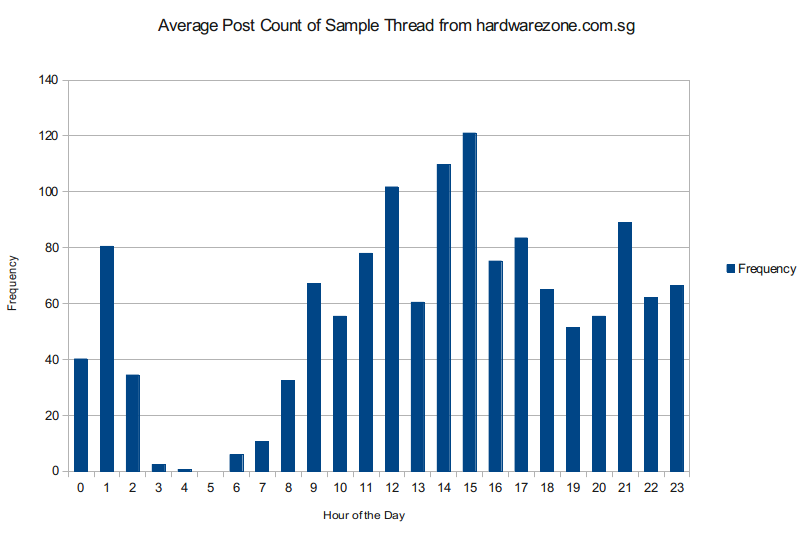
\includegraphics[scale=0.5]{threadfreq.png}}
\caption{The post frequency of a thread from forums.hardwarezone.com.sg shows a pattern cycle of the forum's users.}
\end{figure}
From our initial analysis of the extracted data from the Hardwarezone forums, we have made the following observations about non-sticky threads in the forum:
\begin{enumerate}
	\item There are threads that are very short-lived, and some that are long lived. This is largely dependent on the thread content. For example, a user looking to buy/sell a product that no one has an interest in. %TODO cite paper that shows the lifetime of threads
	\item The long-lived threads typically have a pattern to the frequency of postings. A high frequency of posts are seen around lunch time (12-3 PM) and another spike is seen during the night at 9 PM. (Figure \ref{sleepcycle}). It is yet to be determined if this type of cycle is site-wide or thread-specific.
\end{enumerate}
Our initial model aims to incorporate these observations. A new thread (represented by $q_0$ which only has one post, may transition to either an active or active but `sleeping' thread, or an inactive thread.
%This is to account for the fact that a thread may be active, but the thread has a lack of activity, due to the fact that its' users are sleeping or working.


\begin{figure}
	\begin{center}
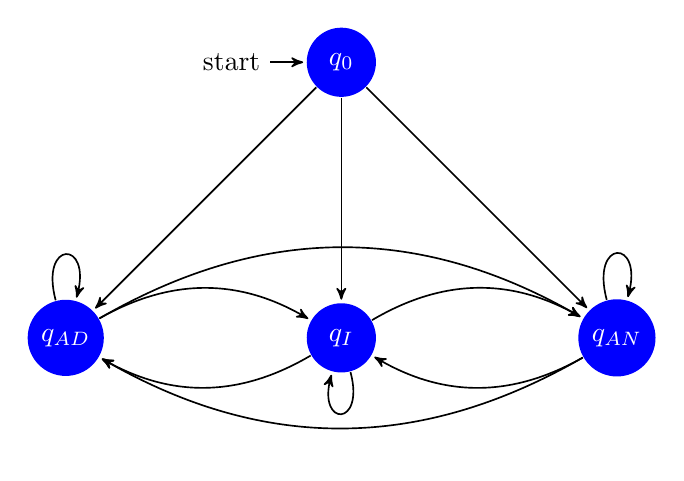
\begin{tikzpicture}[->,>=stealth',shorten >=1pt,auto,node distance=3.5cm,
                    semithick]
  \tikzstyle{every state}=[fill=blue,draw=none,text=white]

  \node[initial,state] (q0)                    {$q_0$};
  \node[state]         (IN) [below of=q0] {$q_I$};
  \node[state]         (AD) [left of=IN] {$q_{AD}$};
  \node[state]         (AN) [right of=IN] {$q_{AN}$};

  \path (q0) edge              node {} (AD)
 			 edge 			   node {} (AN)
			 edge 			   node {} (IN)
		(AD) edge [loop above] node {}(AD)
			 edge [bend left]  node {}(AN)
			 edge [bend left]  node {}(IN)
		(AN) edge [bend left]  node {}(AD)
			 edge [loop above] node {}(AN)
			 edge [bend left]  node {}(IN)
		(IN) edge [bend left]  node {}(AD)
			 edge [bend left]  node {}(AN)
			 edge [loop below] node {}(IN);
\end{tikzpicture}

\end{center}
	\caption{Preliminary modelling of a thread as a probabilistic automaton}\label{spaceship}
\end{figure}
We define active here as threads with a high post frequency, and inactive threads and as posts with low post frequency. Since our observations show that threads have different levels of post frequencies due to usage patterns consistent with user's sleep cycles and work commitment, we use 3 states in total to represent the state of a thread with more than 2 posts. A `day' state (represented by $q_{AD}$) and a `night' state (represented by $q_{ND}$). The inactive threads are represented by the state $q_I$
%Our initial model aims to incorporate these observations. A new thread (represented by $q_0$) which only has one post, may transition into either an active or inactive state (represented by $q_A$ respectively). We define active here as threads with high post frequency, and inactive threads as posts with low post frequency. Since our observations show that threads have different levels of post frequencies due to usage patterns consistent with user's sleep cycles, we use four states in total to represent the state of a thread with more than 2 posts, a `day' state and a `night' state (represented by $q_D,q_N$). These four states form a clique. Each of these states produce a set of observations that we can use to identify the state that a thread is in.

The intuition behind this is the fact that active threads can transition to an inactive state, but the presence of a new post is able to spark off a new discussion within the thread, causing it to be an active thread again.

The graphical representation of this automata is seen in Figure \ref{spaceship}.


Our initial collection of data to identify changes in state for active threads to inactive threads do not show any observable patterns (See Figure \ref{nothing}). More data has to be collected and analysed before conclusions can be made. Statistics of textual content, along with data for a more complete set of threads may provide some insight to their behaviour.

\section{Work to be done}
While much work has already been done, there still remains a substantial amount of implementation and evaluation to be completed. Table \ref{schedule} lays out the schedule for the work left to be done over the holidays.
\begin{table}\label{schedule}
\singlespacing
\begin{tabular}{| l | l | c |}
	\hline
	Start date & End Date & Activity \\
	\hline
	%%%%%%%%%%%%%%%%%%%%%%%%%%%%%%%%%%%%%%%%%%%%%%%%%%%%%%%%%%%%%%%%%%%%%%
%%                                                                  %%
%%  This is a LaTeX2e table fragment exported from Gnumeric.        %%
%%                                                                  %%
%%%%%%%%%%%%%%%%%%%%%%%%%%%%%%%%%%%%%%%%%%%%%%%%%%%%%%%%%%%%%%%%%%%%%%
2012-05-07	&2012-05-11	&Implement feature extraction from threads\\
2012-05-14	&2012-05-18	&Collect more data from other forums\\
2012-05-21	&2012-05-25	&Implement baseline using classification algorithm (SVM)\\
2012-05-28	&2012-06-01	&Implement linear regression from Yang et. Al.\\
2012-06-04	&2012-06-08	&Implement and test HMM\\
2012-06-11	&2012-06-15	&Implement and test HMM\\
2012-06-18	&2012-06-22	&Implement and test HMM\\
2012-06-25	&2012-06-29	&Implement and test HMM\\
2012-07-02	&2012-07-06	&Implement and test HMM\\
2012-07-09	&2012-07-13	&Evaluation\\
2012-07-16	&2012-07-20	&Evaluation\\
2012-07-23	&2012-07-27	&Evaluation\\
2012-07-30	&2012-08-03	&Evaluation\\

	\hline
\end{tabular}
\caption{Schedule for the holidays}
\end{table}
% use weka, do x-fold validation

%\begin{figure}
%	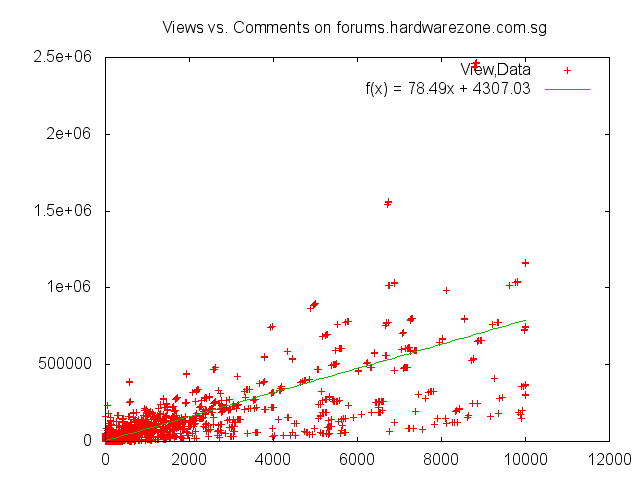
\includegraphics[scale=0.5]{view-comment.png}
%	\caption{Linear fit of Views vs Comments from forum.hardwarezone.com.sg}
%\end{figure}

\bibliographystyle{acm}
\bibliography{report}
\end{document}
